\documentclass[10pt,xcolor=dvipsnames]{beamer}

\usetheme{Frankfurt}
%\usetheme{Bergen}
%\usetheme{Goettingen}
\usepackage{listings}
\usepackage{paralist}
\usecolortheme[RGB={0,104,139}]{structure}%deepskyblue
%\usecolortheme[named=Maroon]{structure}

\title[Cloud based IT Infra with Central Identity]{Cloud based IT Infra with Central Identity}
\subtitle{Phase I}

\author{ \underline{Project Guide} \\ \hspace{2mm} \\ \small{ T. Chandra Shekar } \tiny \\ \underline{} \\ \scriptsize \textit{Lecturer -- Dept. of CSE} }
\institute{ \underline{Presenting by} \\ \hspace{2mm} \\ \textit {Team r3b00+ }  \\ \hspace{4mm} \\ Dept. of CSE, RGUKT -- Nuzvid}
\usepackage{color}
 
\definecolor{codegreen}{rgb}{0,0.6,0}
\definecolor{codegray}{rgb}{0.5,0.5,0.5}
\definecolor{codepurple}{rgb}{0.58,0,0.82}
\definecolor{backcolour}{rgb}{0.95,0.95,0.92}
\lstdefinestyle{mystyle}{
    backgroundcolor=\color{backcolour},   
    commentstyle=\color{codegreen},
    keywordstyle=\color{magenta},
    numberstyle=\tiny\color{codegray},
    stringstyle=\color{codepurple},
    basicstyle=\footnotesize,
    breakatwhitespace=false,         
    breaklines=true,                 
    captionpos=b,                    
    keepspaces=true,                 
    numbers=left,                    
    numbersep=5pt,                  
    showspaces=false,                
    showstringspaces=false,
    showtabs=false,                  
    tabsize=2
}
 
\lstset{style=mystyle}

\AtBeginSection[]
{
	\begin{frame}
		\frametitle{Outline}
		\tableofcontents[currentsection,hideothersubsections]
	\end{frame}
}
%\AtBeginSubsection[] % Do nothing for \subsection*
%{
%\begin{frame}<beamer>
%\frametitle{Outline}
%\tableofcontents[currentsection,]
%\end{frame}
%}

\begin{document}


\begin{frame}
\titlepage
\end{frame}

%\begin{frame}
%\frametitle{Outline}
%\tableofcontents[hideallsubsections]
%\end{frame}

\begin{frame}{About us}

\small
\begin{center}
We are from team \textit{r3b00+}  \{reboot\} \\ \hspace{4cm} \\
\begin{tabular}{l  l }
T. Aneesh Kumar & N090247   \\
P. Nageswarao  & N091030  \\
P. Anesh  & N090977 \\
P. Jyothi Ram & N090990 \\
K. Naresh Chowdary  & N090331 \\
N. Venkata Sateesh  & N090935 \\
M. Sanyasirao & N090891  
\end{tabular}


\end{center}


\end{frame}
 

\section{Objective}
\subsection{Objective}
\begin{frame}{Objective}

Our objective is to create a  private cloud and availing access of all its services using central identity with single sign on through dynamic role based management along with REST API to third party for application developers and users. \newline

This can be developed by using open source tools like OpenStack, NFS, LDAP, Ubuntu and etc \newline

Expecting to serve with virtual machines to the research, virtual labs rather than dedicated lab hardware.
\end{frame}

\subsection{Motivation}
\begin{frame}{Motivation}

\begin{itemize}
	\item No Central Identity, Central Storage \& High capacity hardware resource pool.
	\item Failed to maintain large user load web services like ONB, Exam servers, etc.
	\item Dedicated computer course labs like Matlab, VLSI, etc.
	\item No proper Web Application Security \& Standards.
	\item Inadequate resource requirements for Research.
\end{itemize}

\end{frame}



\section{Proposed System}
\subsection{Users \& IT Services}
\begin{frame}{Users \& IT Services}
We are collaborating all IT Services that are required for University and identifing the users who is going to use them. All Users are catagorized into 4 groups $ ^{[1]}$
	
	\begin{itemize}
	\item Studens, Developers, Staff, faculty \& Researches
	\end{itemize}
\begin{figure}[H]
\begin{center}
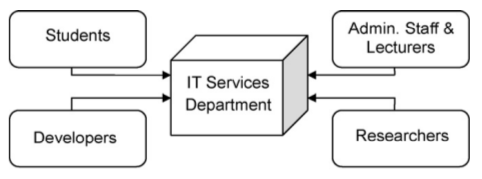
\includegraphics[width=5cm]{./it.png}
\caption{ Simplified structure of the main users of IT services. \label{fig:Simplified structure of the main users of IT services. }}
\end{center}
\end{figure}
	
\end{frame}
\subsection{Cloud Infrastructures}
\begin{frame}{Cloud Infrastructures}
All University IT Services are deployed in a private cloud, constructed over exsiting infrastructure, that can be broadly viewed as 
	
\begin{figure}[H]
\begin{center}
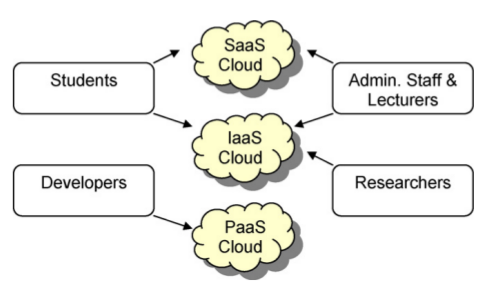
\includegraphics[width=7cm]{./it2.png}
\caption{ IT Services and Users in Cloud Computing\label{fig:IT Services and Users in Cloud Computing }}
\end{center}
\end{figure}	
	
	
\end{frame}

\begin{frame}{Proposed System -  Main Components}
\begin{itemize}
	
	\item Network Components 
	\begin{itemize}
		\item AAA, LDAP, NFS
	\end{itemize}
	\item Central Identiy 
	\begin{itemize}
		\item Single Sign on
		\item Fedarated Identity
		\item Dynamic Role Based Access Control
		\item REST API to third party
	\end{itemize}
	\item Cloud Infrastructure
	\begin{itemize}
		\item Cloud Computing, Private Cloud, Open source tools
	\end{itemize}
\end{itemize}
\end{frame}

\section{Network Components}
\subsection{Introduction}
\begin{frame}{Introduction}
To construct a Campus Area Network(CAN), building network is an important and complex task. So in order to make that complex task easier and very robust in nature we have to use some of these components such as LDAP, AAA and NFS.
\newline

Devices used to setup a Local Area Network (LAN) are the most common types of network devices used by the public. A LAN requires a router, switch, cabling or radio technology, network cards.
\end{frame}

\subsection{Why Network Components?}
\begin{frame}{Why Network Components?}
To build a robust and secure network we must use some of these components in constructing that network. These will simple our manual work by automating many complex tasks and very useful.\linebreak \\
The given below are some basis network components\linebreak \\ 

\subsubsection{Router}
\textbf{Router: }
A router is a device that forwards data packets along networks. A router is connected to at least two networks, commonly two LANs or WANs or a LAN and its ISP's network. Routers are located at gateways.\linebreak \\
\subsubsection{Switch}
\textbf{Switch: }
A network switch is a computer networking device that connects devices together on a computer network, by using a form of packet switching to forward data to the destination device.
\end{frame}
\subsection{AAA, LDAP and NFS Servers}
\begin{frame}{AAA \& LDAP }
\subsubsection{AAA}
\textbf{AAA:}
Authentication, Authorization and Accounting
\begin{itemize}
	\item An AAA server is a server program that handles user requests for access to computer resources and, provides authentication, authorization, and accounting (AAA) services
	\item The current standard by which applications communicate with an AAA server is either RADIUS or TACACS+
\end{itemize}
\underline{}\\
\subsubsection{LDAP}
\textbf{LDAP:}
Lightweight Directory Access Protocol
\begin{itemize}
	\item For accessing and maintaining distributed directory info
	\item LDAP provides a secure way to access information presented in directories by using some authentication methods
\end{itemize}
\end{frame}
\subsubsection{NFS}
\begin{frame}{NFS Servers}
\textbf{NFS:}
Network File System
\begin{itemize}
	\item It is a client/server system that allows users to access files across a network and treat them as if they resided in a local file directory
	\item Exporting: NFS Server provides clients with access to its files
	\item Mounting: File systems are made available to OS and the user	
\end{itemize}

\end{frame}


\section{Single Sign-On}
\subsection{What is SSO}
\begin{frame}{What is Single Sign-On?}
 
\begin{itemize}
	\item Single Sign-On (SSO) is an authentication process that allows a user to access multiple applications with one set of login credentials. 
	\item One login. All of RGUKT.
\end{itemize}

\begin{figure}
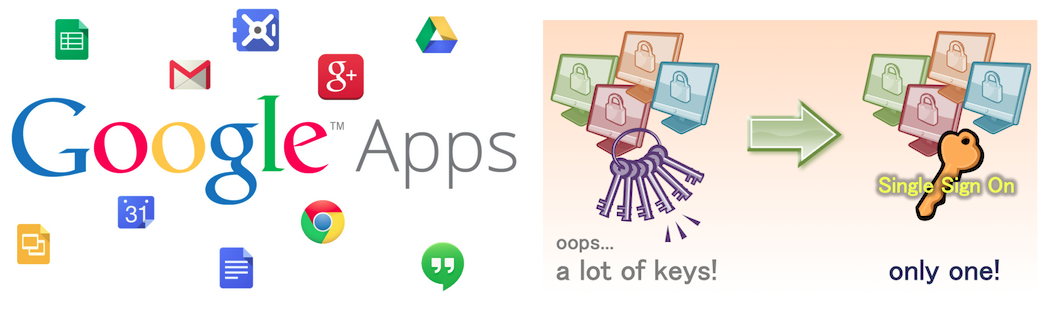
\includegraphics[width=8cm,height=3.5cm]{SSO}
\caption{Google SSO and Application \label{fig:Google SSO and Application}}
\end{figure}

\end{frame}
\subsection{Why SSO}
\begin{frame}{Why Single Sign-On?}

\begin{itemize}
	\item Signing Up everytime is troublesome
	\item I am a nerd, I can't remember all the passwords across multiple Apps.
	\item Is it possible to just sign-on once to perform all the actions?
	\item Is basic Authorization on many sites is secure? Any alternative?
	\item Yes!! Single sign-on can be used to answer all these Questions.
\end{itemize}

\end{frame}

\subsection{Advantages}
\begin{frame}{Advantages}
\begin{itemize}
	\item Ease burden on developers
	\item Improved user experience, no password lists to carry. Thus, improving productivity.
	\item Ease of Access through a single Central Database.
	\item Transfer of Sensitive Data across network is minimized.
	\item Enables users to login quickly and securely to all their applications.
	\item Auditing \& Statistical history reviewing simplified.
\end{itemize}
\end{frame}

\subsection{How well we will implement?}
\begin{frame}{How well we will implement?}
\begin{itemize}
\item We want to develope well structured and documented REST API
\item Designing neat and user friendly interface with Semantic UI
\item Technologies to be Used
\begin{figure}

\includegraphics[width=9.5cm,height=1.5cm]{technologies}
\end{figure}
\item Standards to be followed
\begin{figure}

\includegraphics[width=7cm,height=2cm]{standards}
\end{figure}
\end{itemize}
\end{frame}

\subsection{What is JSON?}
\begin{frame}{What is JSON?}

\textbf{JSON}\\

\begin{itemize}
\item JSON stands for \textbf{J}ava\textbf{S}cript \textbf{O}bject \textbf{N}otation
\item An open standard format that uses plain text to transmit data.
\item Used primarily to transmit data between a server and web application, as an alternative to XML.

\end{itemize}
\textbf{Example}
\lstinputlisting[language=Java,caption=JSON Example]{abc.json}
\end{frame}

\subsection{What is REST?}
\begin{frame}{What is REST?}

\textbf{REST API}

\begin{itemize}
\item REST stand for \textbf{RE}presentational \textbf{S}tate \textbf{T}ransfer
\item A Collection of simple URIs, and HTTP calls to those URIs and some JSON resources
\item Basic CRUD Operations
\end{itemize}

\begin{figure}
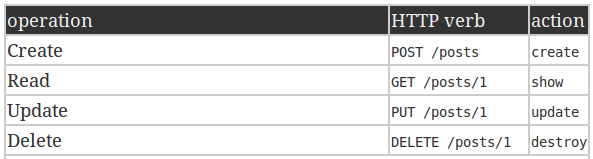
\includegraphics[width=7cm,height=2cm]{CRUD}
\caption{CRUD Operations \label{fig:CRUD Operations}}
\end{figure}

\end{frame}


\subsection{What is REST? (Contd...)}
\begin{frame}{REST API Example}
\textbf{Syntax}
\begin{itemize}
	\item http://it-ebooks-api.info/v1/book/:id/:author/
\end{itemize}
\textbf{Example}
\begin{itemize}
	\item Request URI -- http://it-ebooks-api.info/v1/book/1234/
	\item Response 
\end{itemize}
\lstinputlisting[language=Java,caption=REST Example]{abc2.json}

\end{frame}

\section{Identity Management}
\subsection{Introduction}
\begin{frame}{Introduction}
\begin{itemize}
	\item Users need to Manage different passwords to authenticate at various applications
	\item This is done at a central point to unify the authentication \& authorization
	\item Organization has to take care of it, if not out-source it
	\item \textbf{Different Implementations}
\begin{itemize}
	\item Kerberos, LDAP Servers, Relational db's
	\item X.509 Certificate based, FIdM (Shibboleth)
\end{itemize}
	\item \textbf{Secure Mechanisms}
\begin{itemize}
	\item User-Centric Identity
	\item Federated Identity
\end{itemize}
\end{itemize}
\end{frame}

\subsection{Federated Identity Management}
\begin{frame}{Federated Identity Management}
\begin{itemize}
\item SSO introduced on a large scale with Kerberos protocol
\item SAML = Authentication + Authorization
\item User can get access by using I-Card or Unique URL
\item \textbf{Components}: SP, IdP, Federation(AAI), DS or WAYF Server, X.509 Certificates.

\item \textbf{Advantages}
\begin{itemize}
	\item Secure, Prevalent, Fine-grained Authorization
\end{itemize}
\item \textbf{Disadvantages}
\begin{itemize}
	\item Complexity of the protocol, Unable to manage privacy info
\end{itemize}
\end{itemize}
\end{frame}

\begin{frame}{Federated Identity Management Continued}
\begin{figure}
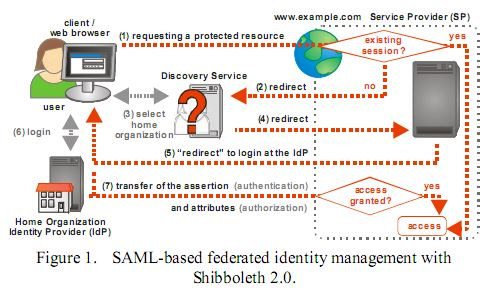
\includegraphics[width=8cm,height=6cm]{fidm}
\end{figure}
\end{frame}

\subsection{User Centric Identity Management}
\begin{frame}{User-Centric Identity Management}
\begin{itemize}
\item The user presents the information as the I-Card
\item There is no need of DS, its done on the user side
\item User can get access by using I-Card or Unique URL
\item \textbf{Components}: I-Card or Unique URL, SP, IdP, etc.
\item \textbf{Advantages}
\begin{itemize}
	\item Usability,More Privacy, Simplification of Protocol
\end{itemize}
\item \textbf{Disadvantages}
\begin{itemize}
	\item Security Risks(Phishing, XSS, CSRF),No single standard 
\end{itemize}
\end{itemize}
\end{frame}

\begin{frame}{User-Centric Identity Management Continued}
\begin{figure}
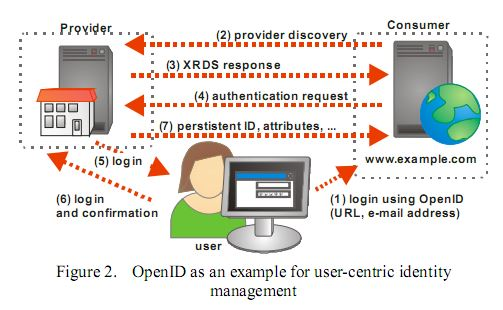
\includegraphics[width=8cm,height=6cm]{ucidm}
\end{figure}
\end{frame}

\subsection{Relating to our University}
\begin{frame}{Intra \& Inter campus Infrastructure}
\begin{columns}
\column{0.4\textwidth}
\begin{figure}[H]
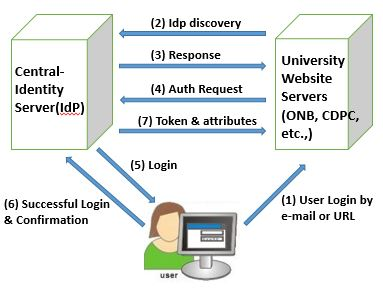
\includegraphics[width=4cm,height=3.5cm]{U1}
\caption{Intra Campus\label{fig:Intra Campus}}
\end{figure}
\column{0.6\textwidth}
\begin{figure}[H]
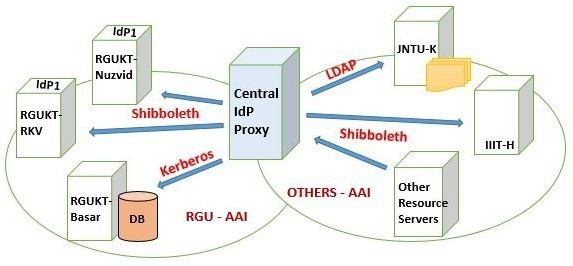
\includegraphics[width=6cm,height=4cm]{ex1}
\caption{Inter Campus\label{fig:Inter Campus}}
\end{figure}
\end{columns}

\end{frame}

\section{RBAC}
\subsection{Introduction}
\begin{frame}{Introduction to RBAC}
\begin{itemize}
 \item Role Based Access Control(RBAC) assigns users to roles and then roles to permissions, It solves problems of least privilege, separation of duty and other security issues
 \item In RBAC model, these rights are defined based on the role that individuals are assigned to in an organization
 \item It overcomes the problems in DAC which is flexible but not secure and MAC which is Secure but not flexible
\end{itemize}
\begin{figure}[H]
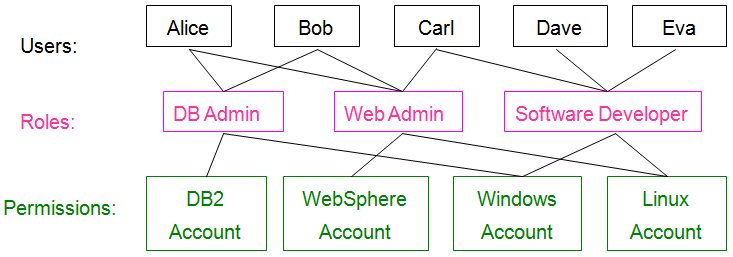
\includegraphics[width=9cm,height=3cm]{sunny1}
\caption{Scenario of RBAC\label{fig:Scenario of RBAC}}
\end{figure}
\end{frame}

\subsection{Idea of RBAC}
\begin{frame}{Basic Idea of RBAC}
\begin{itemize}
	\item  Access Control policy is embodied in various components of RBAC such as,
	\begin{itemize}
	\item Role-Permission relationships
	\item User-Role relationships
	\item Role-Role relationships
	\end{itemize}
	\item Users get roles corresponding permissions by getting roles to operate on the objects
	\item RBAC model is defined in terms of three model components - Core RBAC, Hierarchical RBAC and Constraint RBAC
\end{itemize}
\begin{figure}[H]
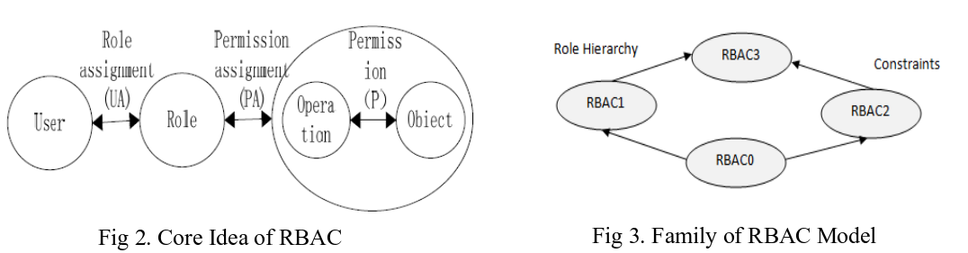
\includegraphics[width=10cm,height=3cm]{sunny2_r}
\end{figure}
\end{frame}
\subsection{Structure of RBAC}
\begin{frame}{Structure Diagram of RBAC Model}
\begin{columns}
 
\column{0.6\textwidth}
\begin{itemize}
\item The Structure diagram of role based access control model consists of role hierarchies and constraints
\item Role hierarchical relationship expresses the inheritance in roles permissions
\begin{itemize}
\item User inheritance
\item Permission inheritance
\item Activation inheritance
\end{itemize}
\item Constraints in RBAC adds separation of duty relations
\begin{itemize}
\item Mutual exclusion
\item Pre-condition
\item Cardinality
\end{itemize}
\end{itemize}
 
\column{0.4\textwidth}
\begin{figure}[H]
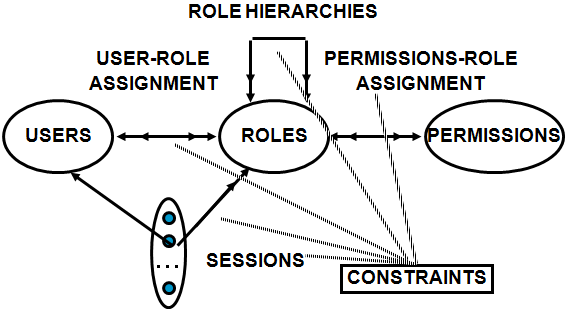
\includegraphics[width=4cm,height=3cm]{sun3}
\caption{RBAC3 Mode}
\end{figure}
\end{columns}
\end{frame}

\subsection{Dynamic RBAC}
\begin{frame}{Dynamic RBAC}

Dynamic RBAC overcomes the shortages of the traditional RBAC by adding with dynamic constraints and  permissions
\begin{itemize}
 \item It retains original static constraints of traditional RBAC
 \item The App creator no need to go for administration, himself he can add or create a role for users
 \item It supports each user has different levels of permission at different time
\end{itemize}
\begin{figure}[H]
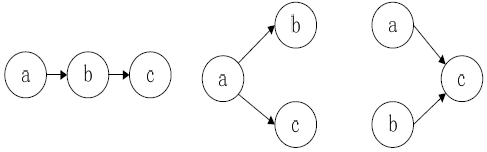
\includegraphics[width=10cm,height=3cm]{ass}
\caption{Different Types of Association}
\end{figure}
\end{frame}



\section{Cloud Infra}
\subsection{Cloud Computing}

\subsubsection{Introduction}
\begin{frame} {Cloud Computing - Introduction }
%One can define Cloud Computing with essential characteristics like
\textbf{What is Cloud Computing ...?} \\
\hspace{4cm} \\
\textit{``Cloud computing is a model for enabling convenient, on-
demand network access to a shared pool of configurable
computing resources (e.g., networks, servers, storage,
applications, and services) that can be rapidly provisioned
and released with minimal management effort or service
provider interaction''} $ ^{[1]} $\newline
\\
\textbf{Essential Characteristics:} \\
\begin{itemize}
\item On-demand self-service
\item Broad network access 
\item Resource pooling 
\item Rapid elasticity 
\item Measured Service 
\end{itemize}
\end{frame}

\subsubsection{Servcice & Deployment Models}
\begin{frame}{Cloud Computing - Servcice \& Deployment Models }
\textbf{Servcice Models:} \\ 
\begin{figure}[H]
 \centering
 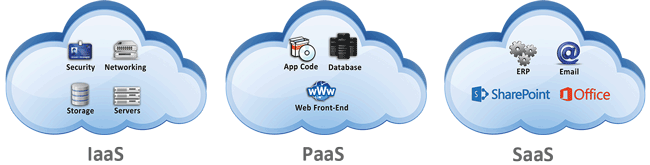
\includegraphics[width=7cm,height=1.75cm]{./service.png}
 \caption{Cloud Computing - Servcice Models \label{fig:Cloud Computing - Servcice Models} }
\end{figure}

\textbf{Deployment Models:} \\ 

\begin{figure}[H]
 \centering
 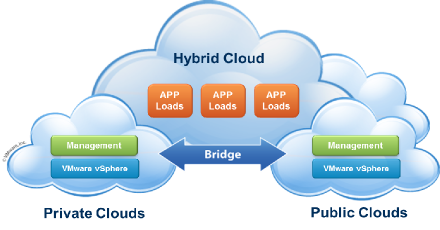
\includegraphics[width=4cm,height=2.5cm]{./model.png}
 \caption{Cloud Computing - Deployment Models \label{fig:model} }
\end{figure}
\end{frame}

\subsection{Private Clouds}

\begin{frame}{Private Clouds -- Definition \& Opensource Tools }
\textbf{``Private Cloud''} \\ 
\hspace{16mm} -- \textit{It is one of the cloud deployment model where the resources of small or medium organization are united and cattered to users of the that organization or outsourced through internet.}\newline \\
\textbf{Opensource Tools:} \\ 
\begin{figure}[H]
 \centering
 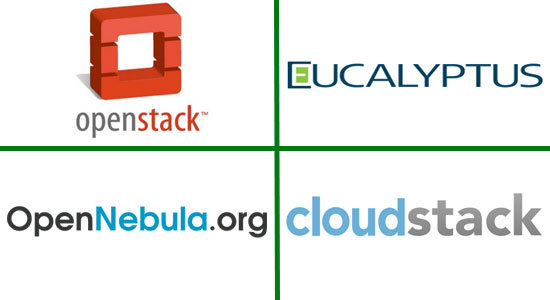
\includegraphics[width=5cm]{./cloud.jpg}
 \caption{Private Cloud - Open source tools \label{fig:cloud} }
\end{figure}
\end{frame}

\subsection{Cloud Infrastructure}
\begin{frame}{Architecture}
\begin{figure}[H]
 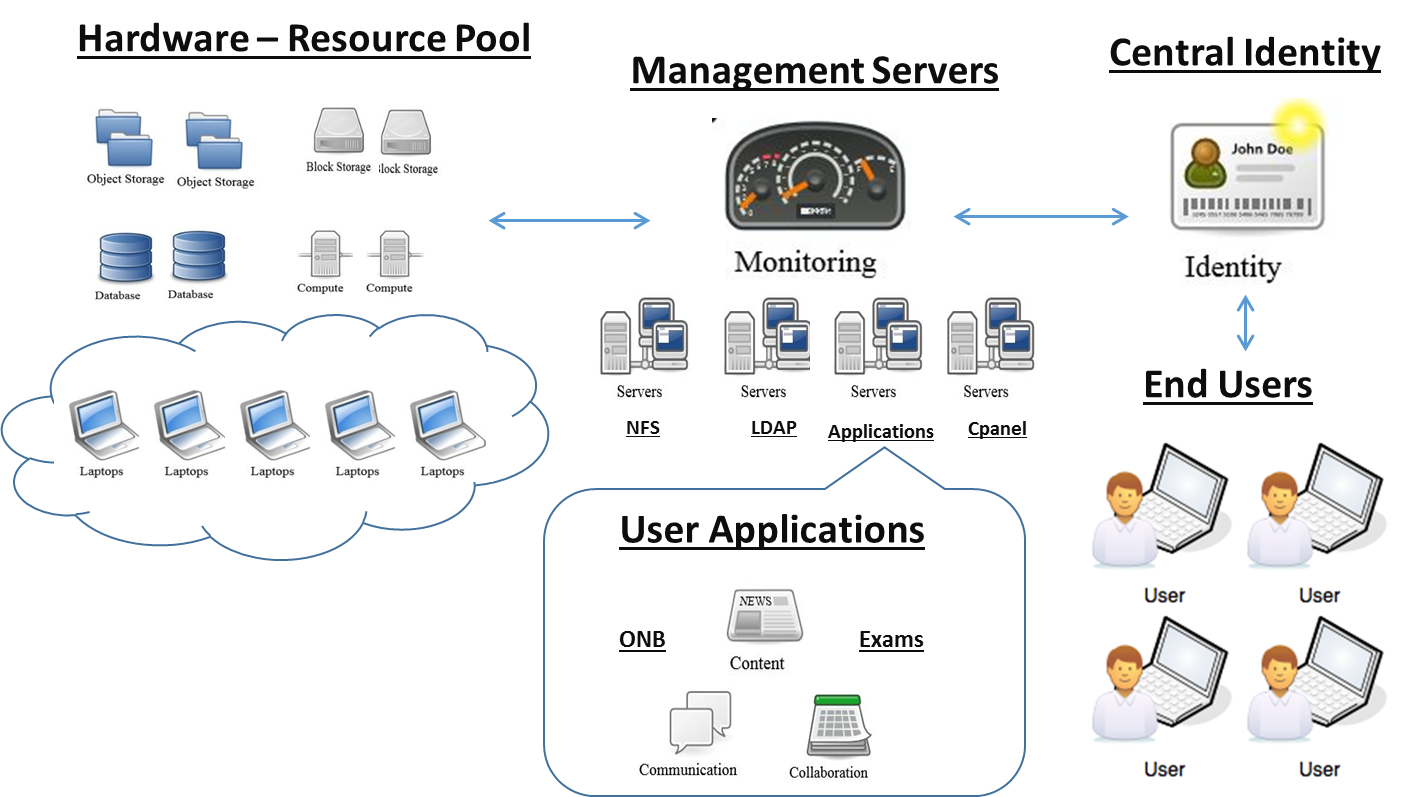
\includegraphics[height=6cm]{./all.png} \\ 
\caption{Cloud Infrastructure Archtitecture} 
\end{figure}
\end{frame}
\section*{References}
\small
\begin{frame}{References}
\begin{itemize}
\item Nabil Sultan, ``Cloud Computing for Education”, International journal information management, 30, pp 109-116, 2010.
\item Tharam Dillon, Chen Wu and Elizabeth Chang, ``Cloud Computing: Issues and Challenges'',  24thIEEE International Conference on Advanced Information Networking and Applications, 2010 
\item Sebastian Rieger, ``User-centric Identity Management in Heterogeneous Federations'', Fourth international conference on Internet and Web Applications and Services, 2009.
\item Jun Zheng, Qikun Zhang ,Shangwen Zheng and Yuan Tan, ``Dynamic Role Based Access Control'',  JOURNAL OF SOFTWARE, VOL. 6, NO. 6, JUNE 2011.
\item R. S. Sandhu, E. J. Coyne, H. L. Feinstein, and C. E.Youman, "Role-Based Access Control Models," [C] IEEE Computer, vol. 29, pp. 38-47, 1996.

\end{itemize}
\end{frame}


\begin{frame}{References}
\small
\begin{itemize}
\item Ivan Novakov, ``Web Single Sign On Systems'', CESNET technical report number 21/2006
\item C.S.Yang, C.Y.Liu, J.H.Chen, C.Y.Sung, ``Design and Implementations of Secure Web-based LDAP Management System''.
\item Ning Li, Qing Wang, Zhongliang Deng, ``Authentication Framework of IIEDNS Based on LDAP and Kerberos'', Proceedings of IC-BNMT2010.
\item Salah A.Jaro Alabady, ``Design implementation of Network Security Model Using Static VLAN and AAA Server
\item Shengli Liu, Wenbing Wang, Yuefei Zhu, ``A New-Style Domain Integrated Management of Windows and UNIX'', The Ninth International Conference on Web-Age Information Management.
\end{itemize}
\end{frame}

\begin{frame}{References}
\small
\begin{itemize}
\item Ubnutu OS, http://www.ubuntu.com/
\item Openstack, https://openstack.org/
\item Linux Bible, http://tuxnetworks.blogspot.com
\item OAuth 2.0, http://oauth.net/
\item Node.js https://nodejs.org
\item Git, https://github.com
\item Bootstrap, http://getbootstrap.com 
\item Stack Overflow http://stackoverflow.com/
\end{itemize}
\end{frame}

\begin{frame}{End}
Thank you and Any Queries ?
\end{frame}

\end{document}